\documentclass[border=10pt]{standalone}

\usepackage{tikz}
\usepackage{tikzsymbols}
\usetikzlibrary{calc,patterns,shapes.geometric}

\def\centerarc[#1](#2)(#3:#4:#5){\draw[#1] ($(#2)+({#5*cos(#3)},{#5*sin(#3)})$) arc (#3:#4:#5);}

\begin{document}
	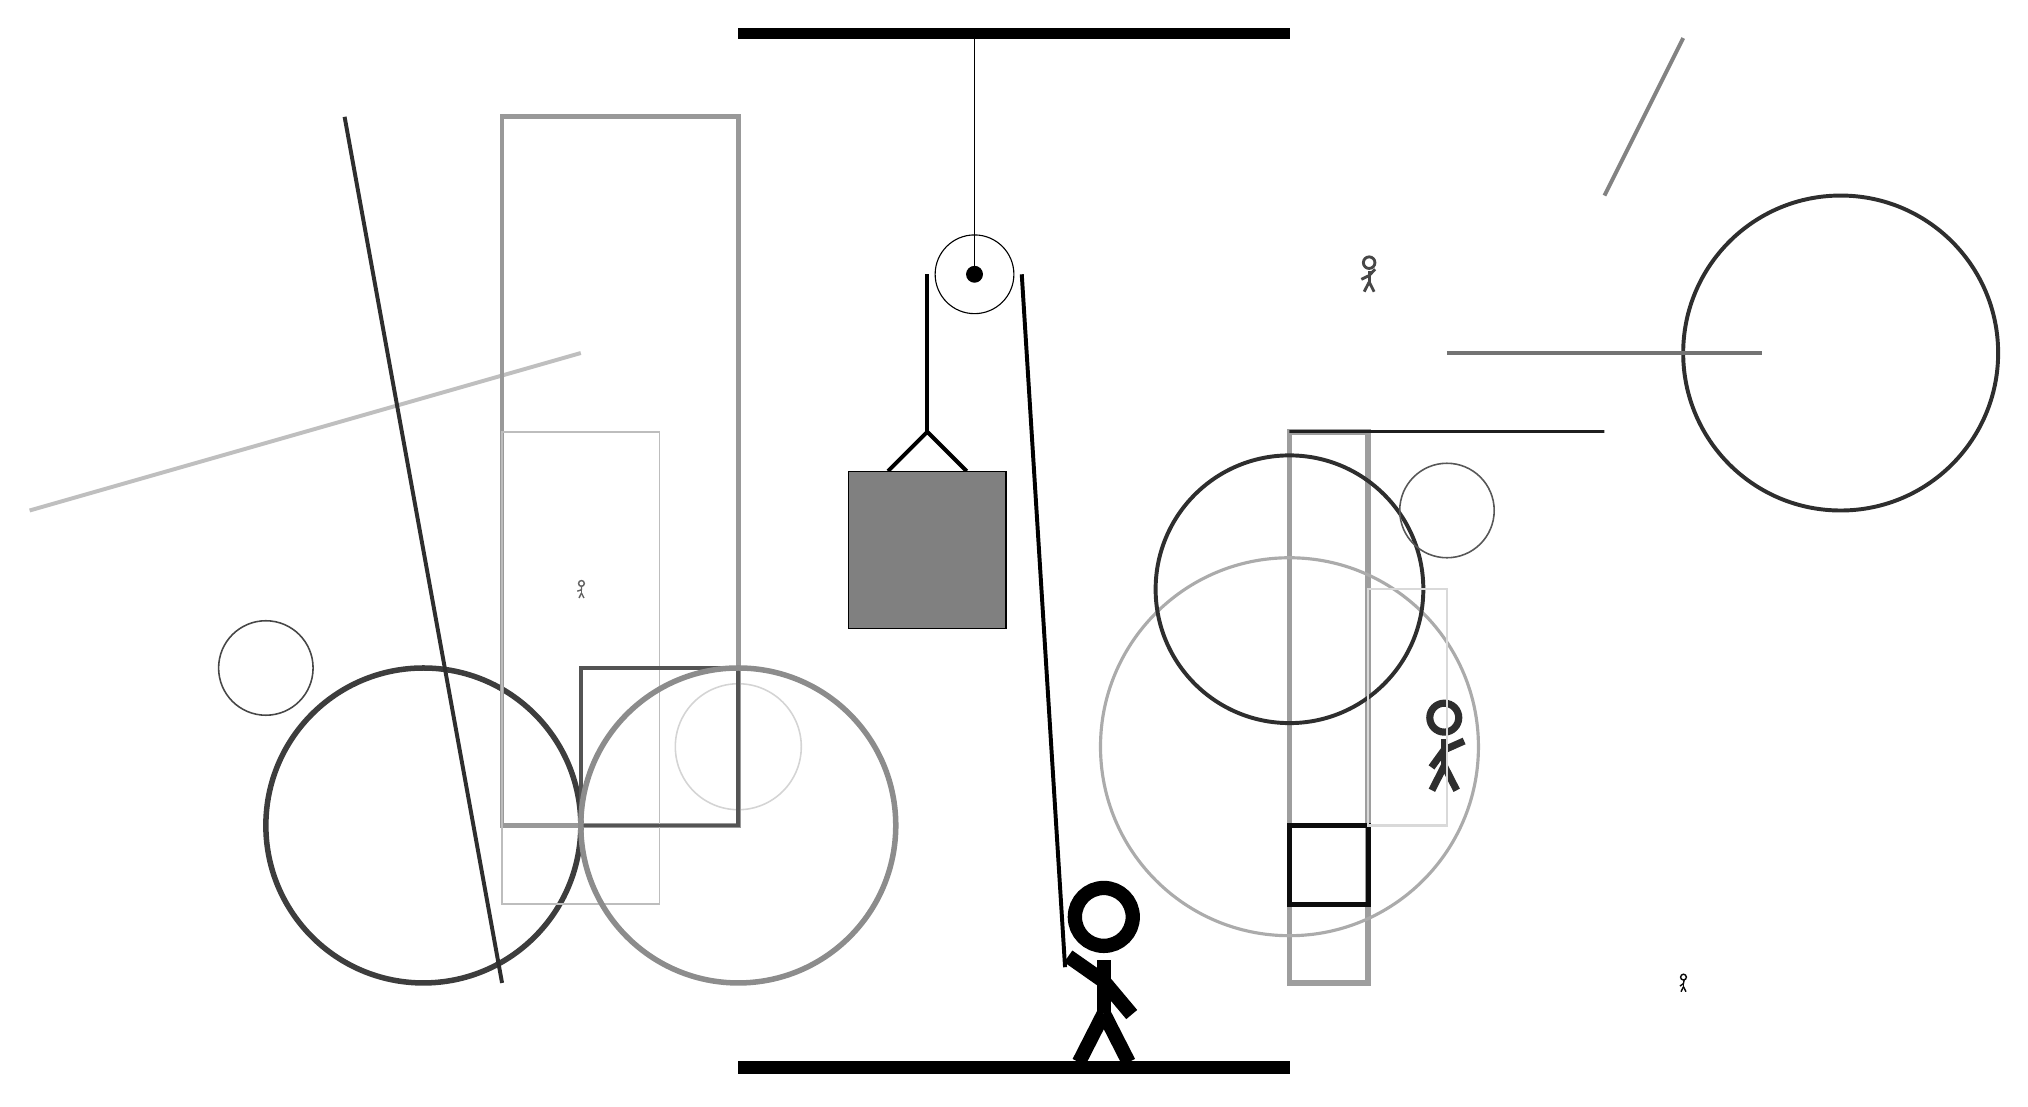
\begin{tikzpicture}
		%%%%% START %%%%%
		
		\draw[fill=black] (-2, 10) rectangle (5, 10.125);
		
		\draw (1, 7) circle (0.5);
		\draw[fill=black] (1, 7) circle (0.1);
		\draw (1, 10) -- (1, 7);
		
		\draw[line width=0.5mm] (-0.1, 4.5) -- (0.4, 5.0) -- (0.9, 4.5);
		\draw[fill=black!50] (-0.6, 4.5) rectangle (1.4, 2.5);
		
		\draw[line width=0.5mm] (0.4, 7) -- (0.4, 5.0);
		\centerarc[line width=0.5mm](1, 7)(0:180:0.6);
		\draw[line width=0.5mm](1.6, 7) -- (2.15, -1.8);
		
		\node at (2.6, -1.9) {\Strichmaxerl[10][-35][-50]};
		
		\draw[line width=0.7mm, color=black!38] (5, 5) rectangle (6, -2);
		
		\draw [line width=0.7mm, color=black!76](-6, 0) circle (2.0);
		\node[line width=0.3mm, color=black!72] at (6, 7) {\Strichmaxerl[2][26][47]};
		\draw [line width=0.2mm, color=black!72](-8, 2) circle (0.6);
		\draw [line width=0.4mm, color=black!33](5, 1) circle (2.4);
		\draw [line width=0.5mm, color=black!82](12, 6) circle (2.0);
		\draw[line width=0.5mm, color=black!25](-4, 6) -- (-11, 4);
		\draw [line width=0.5mm, color=black!82](5, 3) circle (1.7);
		\draw[line width=0.5mm, color=black!82](-7, 9) -- (-5, -2);
		
		\draw [line width=0.3mm, color=black!57](-9, 6) circle (0.0);
		
		\node[line width=0.3mm, color=black!82] at (7, 1) {\Strichmaxerl[5][54][24]};
		\draw [line width=0.2mm, color=black!17](-2, 1) circle (0.8);
		\node[line width=0.6mm, color=black!96] at (10, -2) {\Strichmaxerl[1][36][80]};
		\draw[line width=0.6mm, color=black!40] (-2, 9) rectangle (-5, 0);
		\draw [line width=0.2mm, color=black!66](7, 4) circle (0.6);
		\draw[line width=0.4mm, color=black!88] (5, 5) rectangle (9, 5);
		\draw[line width=0.5mm, color=black!49](10, 10) -- (9, 8);
		
		\draw[line width=0.2mm, color=black!26] (-3, 5) rectangle (-5, -1);
		\draw[line width=0.5mm, color=black!28](7, 3) -- (7, 3);
		\draw[line width=0.6mm, color=black!95] (5, 0) rectangle (6, -1);
		\draw[line width=0.5mm, color=black!67] (-4, 0) rectangle (-2, 2);
		\draw[line width=0.5mm, color=black!55](7, 6) -- (11, 6);
		
		\draw [line width=0.7mm, color=black!45](-2, 0) circle (2.0);
		\node[line width=0.3mm, color=black!61] at (-4, 3) {\Strichmaxerl[1][17][89]};
		\draw[line width=0.3mm, color=black!15] (7, 0) rectangle (6, 3);
		
		
		\draw[fill=black] (-2, -3) rectangle (5, -3.15);
		
		%%%%% END %%%%%
	\end{tikzpicture}
\end{document}